\chapter{System Tests}
\label{chap:6}

In this chapter, the tests  conducted to measure how well the system measures to the
original goals and objectives set out in Section \ref{chap:1}. 

The tests conducted are the voltage and current limits of the relay switches and user
stories where scenarios are created and the response of the system is given. 

\section{Transistor Switch}

MOET NOG GEDOEN WORD

\subsection{Current and Voltage Limits}

MOET NOG GEDOEN WORD

\section{User Tests}

The functionality of the system is tested by exposing it to different user scenarios and
seeing what the outcome is. These tests are performed and discussed in this section.

\subsection{Test 1}

In this user story, the customer decides to pay with a Quick Response Code (QR Code).
He/she does not yet have a user account on the database and has no credits laoded. Figure
\ref{fig:test1} shows the user story. 

The process is as follows: The user first selects which product to buy from the Raspberry
Pi's User Interface (GUI). The Pi then generates a Quick Response Code (QR Code) that the
user scans with any barcode scanning application. The Universal Resource Locator (URL)
embedded in the QR Code then takes the customer to a web page located on the server. 

Not having a user account, the user clicks on the lick to create a new user profile. After
entering valid user information, the customer is returned to the login  page where he/she
can log in with his new login credentials. 

After logging in, the server displays to the customer that he/she does not yet have any
credits loaded onto his account. The customer then goes to the load credit page where
they load some money. When this is done, the server displays a confirmation QR Code on
the customer's cellphone screen, verifying the transaction.

The customer then presses the continue button on the GUI, which starts scanning the web
cam feed for the customer's QR Code. After this is done, the Pi activates the correct
motor and dispenses the product.

\begin{figure}
 \centering 
 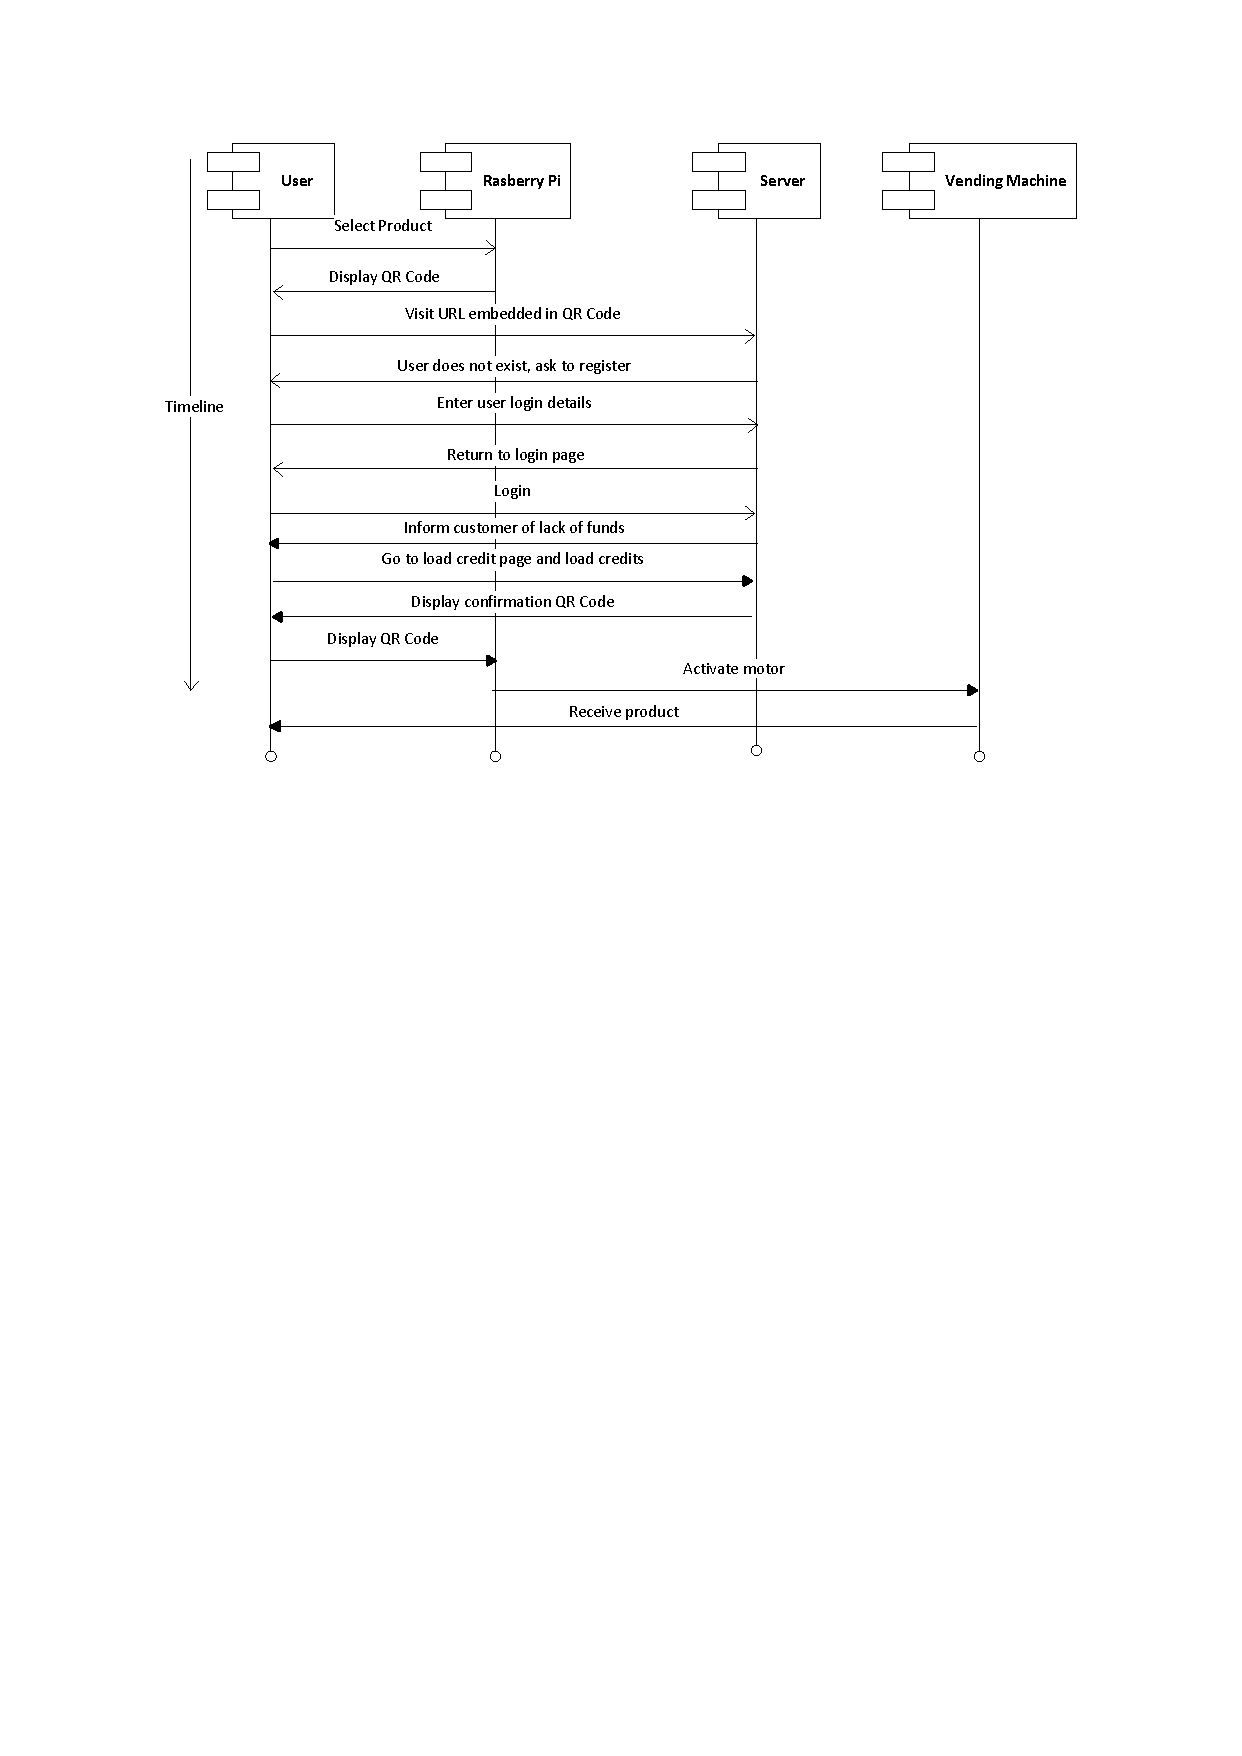
\includegraphics[clip=true, trim = 0 470 0 50,
 scale=0.7]{user_story_1}
 \caption{The first user scenario}
 \label{fig:test1}
\end{figure}

\subsection{Test 2}

In this scenario, a customer tries to use a QR Code from a previous transaction. Figure
\ref{fig:test2} shows the user story.

To begin, the customer selects a product to buy, after which the Raspberry Pi displays a
QR Code. However, instead of scanning the QR Code and paying for a new product, the
customer tries to use an old QR Code that the server sent him/her after a successful
transaction previously. 

The customer tells the Raspberry Pi to scan his old QR Code. The Raspberry Pi does
this, but the old QR Code does not contain a valid response to the Raspberry Pi's
challenge. Therefore, the transaction is valid and the customer is informed of his
invalid QR Code.

\begin{figure}
 \centering 
 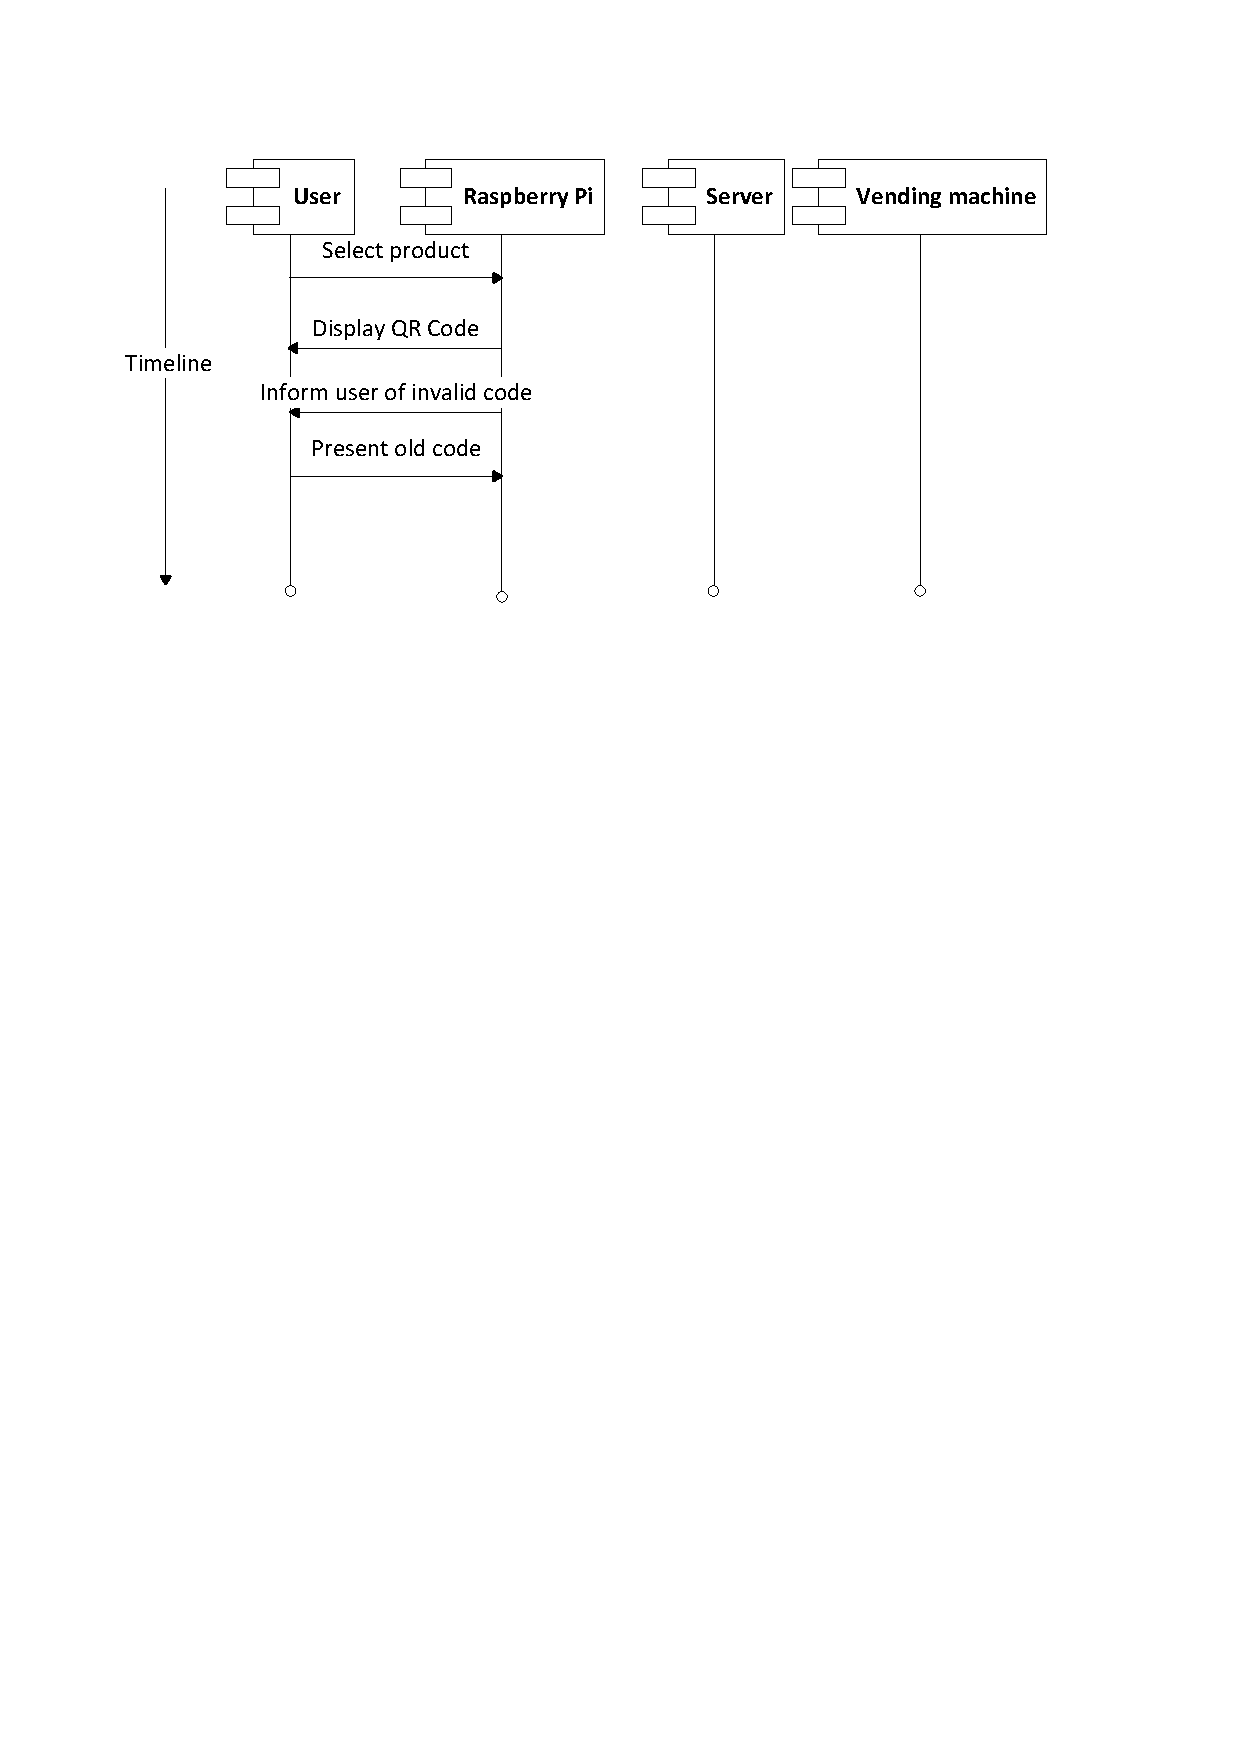
\includegraphics[clip=true, trim = 0 620 0 50,
 scale=0.7]{user_story_2}
 \caption{The second user scenario}
 \label{fig:test2}
\end{figure}

\subsection{Test 3}

In this scenario, the user opts to buy a product using the Android Near Field
Communication (NFC) app. However, a new user profile must first be created. The user story
can be seen in Figure \ref{fig:test3}.

After the user opens the app, he/she is presented with a login screen. The user enters
his login credentials and checks the box that confirms that he/she is a new user. The
app then contacts the server with a user creation request. Provided that the username is
not already in use, the server sends the app a confirmation.

The app then returns the user to the main menu where the user can pick a product to buy.
After picking a product, the app contacts the server with a purchase request. If the
transaction is successful, the server sends the app a confirmation code which the app 
transmits via the cellphone's NFC antenna. 

The user then swipes his phone across the vending machines NFC receiver. The vending
machine then activates the motor and the user receives his product. 

\begin{figure}
 \centering 
 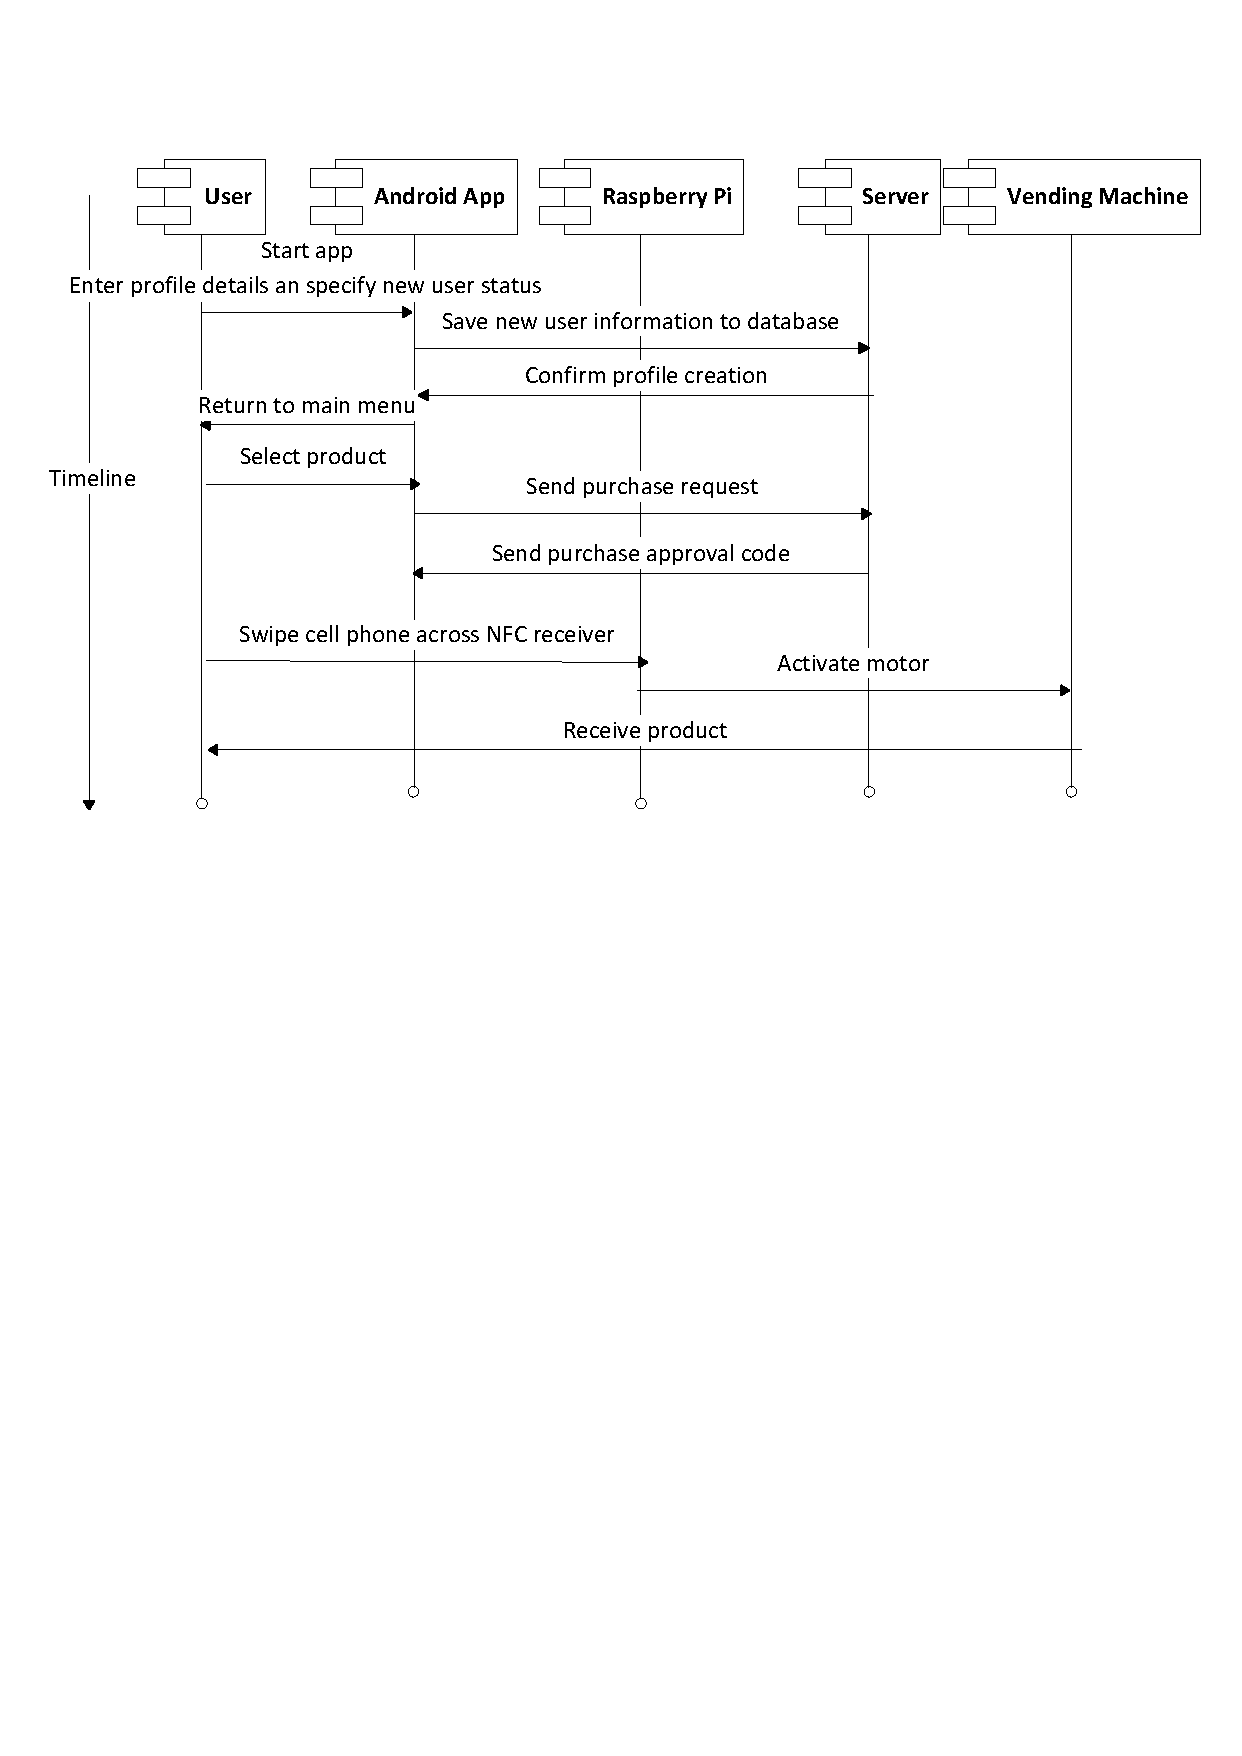
\includegraphics[clip=true, trim = 0 500 0 50,
 scale=0.7]{user_story_3}
 \caption{The third user scenario}
 \label{fig:test3}
\end{figure}